\setAuthor{Jaan Kalda}
\setRound{lahtine}
\setYear{2022}
\setNumber{G 6}
\setDifficulty{6}
\setTopic{TODO}

\prob{Saun}
Subjektiivset palavusetunnet kuumas õhus kirjeldab väga hästi see, kui palju erineb kastepunkt keha temperatuurist. Kastepunkt on temperatuur, mille juures antud õhust hakkab vesi välja kondenseeruma (eeldusel, et rõhk püsib võrdne atmosfäärirõhuga). Olgu leiliruumi õhutemperatuur $T_l=\SI{100}{\celsius}$, saunaõhu kastepunkt $T_k=\SI{10}{\celsius}$ ja leiliruumi ruumala $V=\SI{10}{m^3}$. Mitme kraadini kerkib kastepunkt, kui leiliks vistakase $m=\SI{200}g$ vett? Universaalne gaasikonstant $R=\SI{8.31}{\joule\per\kelvin\per\mole}$; vee molaarmass $\mu=\SI{18}{\gram \per \mole}$.
\begin{center}
    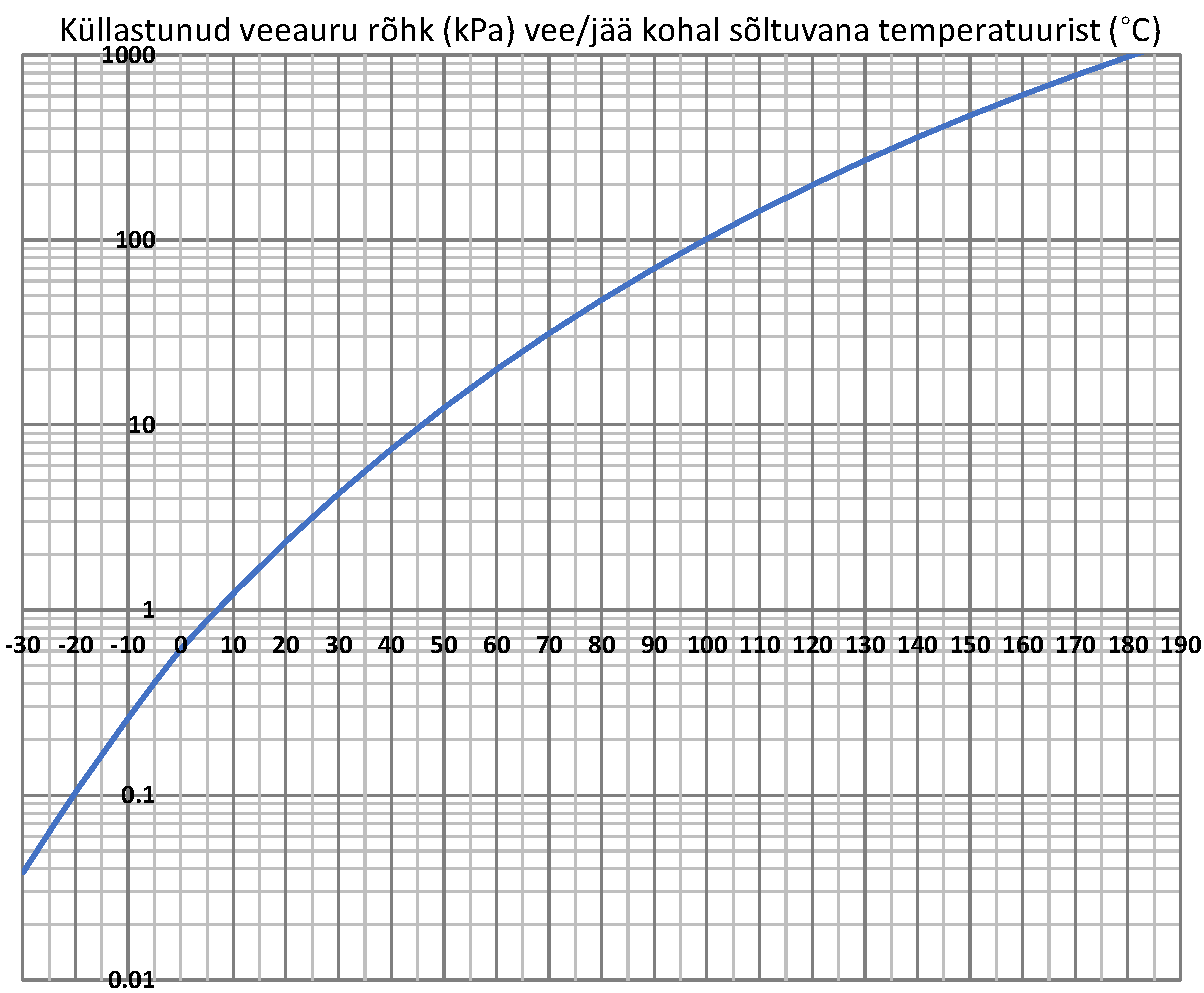
\includegraphics[width=\textwidth]{2022-lahg-06-yl.pdf}
\end{center}




\hint

\solu
Lahendus. Graafiku abil leiame veeauru osarõhu enne leili viskamist $p_a=\SI{1.2}{kPa}$. Ideaalse gaasi olekuvõrrandi abil leiame lisandunud aururõhu $p_bV=\frac m\mu RT$, millest $p_b=\frac {mRT}{\mu V}=\approx \SI{3.4}{kPa}$. Seega veeauru kogurõhk peale leili viskamist $p=p_a+p_b=\SI{4.6}{kPa}$; graafiku abil leiame sellele vastava kastepunkti väärtuse $t_k\approx \SI{32}\celsius$.
\probend